%% Exams

% Software Architecture

\newcommand{\qSoftwareArchitectureOne}{
\begin{ClosedQuestion}
  Consider that a software development team uses an agile methodology
  such as XP (Extreme Programming), where no documentation is
  produced.  Then, the systems developed by that team

    \optionA{Typically have a software architecture that results
    from the common knowledge about the system that is shared among
    the team members}
    \optionB{Do not have a software architecture, because in agile
    methodologies there is no architectural design phase}
    \optionC{Do not have a software architecture, because the practice of
    refactoring allows changing every part of the system easily}
    \optionD{May have a software architecture, but that architecture is
    not known because it was neither designed nor documented}
 \putOptions 
\end{ClosedQuestion}
}

\newcommand{\qSoftwareArchitectureTwo}{
\begin{ClosedQuestion}
  The software architecture of a system

  \optionA{Is a high-level view of the system with the purpose of
  understanding what are the system's goals and features}
  \optionB{Is composed of things such as code units, runtime elements,
  hardware, and people, together with the relationships among them}
  \optionC{Is a set of guidelines that the developing team should
  follow in the development of the system}
  \optionD{Is a set of diagrams that show the runtime elements of the
  system and their relationships}
 \putOptions 
\end{ClosedQuestion}
}


% General scenarios 

\newcommand{\qRequirementsImpact}{
\begin{ClosedQuestion}
	The requirements impact on how an architecture is designed

    \optionA{However, functional requirements do not have any impact on the architecture because the systemic qualities of an architecture are non-functional}
    \optionB{The functional requirements have a large impact on the definition of views of the component-and-connector viewtype because each component executes a functionality}
    \optionC{The functional requirements have a large impact on the definition of views of the module viewtype because they are used to define the high cohesion and low coupling of modules}
    \optionD{The functional requirements can be considered as constraints on the software architecture design}
 \putOptions 
\end{ClosedQuestion}
}


\newcommand{\qConcreteScenarios}{
\begin{ClosedQuestion}
  As part of the process of creating an architecture, we talked about
  a framework for capturing some of the requirements for a system.  In
  this context, \textbf{concrete scenarios} are used for

  \optionA{Describing what are the qualities that the system should possess}
  \optionB{Describing a set of steps that a user of the system must
  perform to accomplish some task}
  \optionC{Describing a use case for the system that makes clear what
  should be the system's responses to each of the user's inputs}
  \optionD{Describing the system's features by way of different
  usage scenarios for it, in which users play the role of actors}
 \putOptions 
\end{ClosedQuestion}
}

% Availability scenario

\newcommand{\qAvailabilityScenarioOne}{
  \begin{ClosedQuestion}
	  Consider the following scenario
	  
	  \begin{quote}
		  If one of the application servers fails to respond when the system is in its normal operation state, the load balancer should redirect requests to another application server.
	  \end{quote}
	  
      \optionA{The stimulus is incorrect response}
      \optionB{The artefact is the load balancer}
      \optionC{The response is not correctly stated}
      \optionD{The quality it addresses is interoperability} 
	  
     \putOptions
% Resposta: C
   \end{ClosedQuestion}
}

\newcommand{\qAvailabilityScenarioTwo}{
  \begin{ClosedQuestion}
	  Consider the following availability scenario
	  
	  \begin{quote}
		 If one of the application servers fails to respond to a request when the system is in its normal operation state, the system should notify the operator and continue to operate normally.
	  \end{quote}
	  
      \optionA{The scenario is not correct}
      \optionB{The scenario is correct but it does not describe whether the request the servers fails to respond to succeeds or fails}
      \optionC{The scenario is correct but it is not clear what is the artefact}
      \optionD{The scenario is not completely correct because it contains two responses} 
	  
     \putOptions
% Resposta: C
   \end{ClosedQuestion}
}

% Availability tactic

\newcommand{\qAvailabilityVotingEN}{
  \begin{ClosedQuestion}
	  The availability quality can be supported by a voting tactic in order to identify faults of

      \optionA{Programming, if the components execute modules developed by different teams}
      \optionB{Hardware, if there is hardware redundancy}
      \optionC{Operating Systems, if redundant components execute on top of different operating systems}
      \optionD{All the previous options} 
	  

     \putOptions
% Resposta: D
   \end{ClosedQuestion}
}

\newcommand{\qAvailabilityOne}{
  \begin{ClosedQuestion}
    There are several tactics to satisfy availability requirements,
    which may be applied depending on the concrete requirement that we
    want to satisfy.  Assuming that you want to deal with faults of type
    \emph{omission} in your system, which tactic is more adequate?

    \optionA{Retry}
    \optionB{Active redundancy}
    \optionC{Ignore faulty behaviour}
    \optionD{Ping/Echo}

    \putOptions

% Resposta: A
 \end{ClosedQuestion}
}


% Performance scenario

\newcommand{\qMWResourceLoaderTacticEEEN}{
  \begin{ClosedQuestion}
	  Consider the following fragment of the \emph{MediaWiki} system description:
	  \newline
	  
	  \emph{To optimize the delivery of JavaScript and CSS assets, the ResourceLoader module was developed to optimize delivery of JS and CSS. Started in 2009, it was completed in 2011 and has been a core feature of MediaWiki since version 1.17. ResourceLoader works by loading JS and CSS assets on demand, thus reducing loading and parsing time when features are unused, for example by older browsers. It also minifies the code, groups resources to save requests, and can embed images as data URIs}
	  \newline
	  
	  The \emph{ResourceLoader} supports a quality
    
    \optionA{Performance}
    \optionB{Usability}
    \optionC{Availability}
    \optionD{Modifiability} 

     \putOptions
   \end{ClosedQuestion}
}

\newcommand{\qInfinispanThree}{
\begin{ClosedQuestion}
	Consider the following description of the \emph{Infinispan} system:
	
	\begin{quote}
		Before putting data on the network, application objects need to be serialized into bytes so that they can be pushed across a network, into the grid, and then again between peers. The bytes then need to be de-serialized back into application objects, when read by the application. In most common configurations, about 20\% of the time spent in processing a request is spent in serialization and de-serialization.
	\end{quote}
	
	The above description can motivate a scenario for
		
    \optionA{Performance}
    \optionB{Availability}
    \optionC{Modifiability}
    \optionD{Reliability}
 \putOptions 
\end{ClosedQuestion}
}


% Performance tactic

\newcommand{\qPerfomanceTacticOne}{
  \begin{ClosedQuestion}
   In which performance tactic it may occur that not all the inputs are processed

    \optionA{Manage sampling rate}
    \optionB{Limit event response}
    \optionC{Reduce overhead}
    \optionD{Bound execution times}

    \putOptions

% Resposta: A
 \end{ClosedQuestion}
}


\newcommand{\qPerfomanceTacticTwo}{
  \begin{ClosedQuestion}
   In which performance tactic it can occur that the inputs are not completely processed, even though they always start being processed

    \optionA{Manage sampling rate}
    \optionB{Limit event response}
    \optionC{Reduce overhead}
    \optionD{Bound execution times}

    \putOptions

% Resposta: D
 \end{ClosedQuestion}
}


% Modifiablity scenario

\newcommand{\qScalabilityINGLES}{
  \begin{ClosedQuestion}
    Several of the cases studied in this course had scalability
    requirements.  That means that those systems should be designed in
    such a way that they

    \optionA{Have high throughput}
    \optionB{Have low latency}
    \optionC{Allow many simultaneous users}
    \optionD{May be easily changed to increase their performance}

    \putOptions

% Resposta: D
 \end{ClosedQuestion}
}

\newcommand{\qModifiabilityScenario}{
  \begin{ClosedQuestion}
    Consider the following modifiability scenario
	
	\begin{quote}
		The effort necessary to successfully port the system to execute in a new browser should not be higher than 5 person/month.
	\end{quote}

    \optionA{The stimulus is to port the system to a new browser}
    \optionB{The environment is build time}
    \optionC{The response is 5 person/month}
    \optionD{To implement the above scenario it is necessary to apply a runtime defer binding tactic}

    \putOptions

% Resposta: A
 \end{ClosedQuestion}
}


% Modifiablity tactic

\newcommand{\qLayersTactics}{
  \begin{ClosedQuestion}
    The main tactic associated with the layered architectural style is:

    \optionA{Split module}
    \optionB{Encapsulate}
    \optionC{Restrict dependencies}
    \optionD{Defer binding}

    \putOptions

% Resposta: C
 \end{ClosedQuestion}
}

\newcommand{\qAspectsTactics}{
  \begin{ClosedQuestion}
    The main tactic associated with the aspects architectural style is:

    \optionA{Split module}
    \optionB{Increase semantic coherence}
    \optionC{Restrict dependencies}
    \optionD{Defer binding}

    \putOptions

% Resposta: B
 \end{ClosedQuestion}
}

% Hadhoop - Scenario

\newcommand{\qHadoopDisponibilidadeDadosINGLES}{
  \begin{ClosedQuestion}
    One of the key requirements for the HDFS system is that the data
    stored in the system remains available, even in the presence of
    various types of failures (non simultaneous) in the hardware in
    which the system executes.  To show that the system satisfies this
    requirement

    \optionA{We must use various different views, both of the
      component-and-connector and the allocation viewtypes}
    \optionB{We just have to show, through component-and-connector
      views, that the system maintains replicas of the data in
      different components}
    \optionC{We just have to show, through Deployment views,
      that the \emph{DataNode} component executes in more than one
      machine of the cluster}
    \optionD{We just have to show, through Decomposition views, that
      there are modules responsible for the replication of file blocks}
    \putOptions

% Resposta: A
  \end{ClosedQuestion}
}

\newcommand{\qHadoopStakeholdersEurosINGLES}{
  \begin{ClosedQuestion}
    In the HDFS system, in the stakeholders perspective, the use of low cost servers to build the clusters is:

    \optionA{Essential to ensure the system scalability}
    \optionB{Essential to reduce costs whenever there is a fault in a hardware element}
    \optionC{Essential to ensure the system portability}
    \optionD{Essential to facilitate the integration with legacy systems}

    \putOptions
% Resposta: B
\end{ClosedQuestion}
}


% Hadhoop - Tactic

\newcommand{\qHadoopTacticasRecuperacaoFaltasINGLES}{
  \begin{ClosedQuestion}
    In the HDFS system the fault recovery tactics are:

    \optionA{Active replication and passive replication}
    \optionB{Active replication, passive replication, and spare}
    \optionC{Passive replication and spare}
    \optionD{Quorum, active replication, and passive replication}
    \putOptions
% Resposta: C
  \end{ClosedQuestion}
}

\newcommand{\qHadoopHeartbeatINGLES}{
  \begin{ClosedQuestion}
    In HDFS, during normal operation DataNodes use the heartbeat tactic

    \optionA{Because this tactic simplifies the addition and removal of DataNodes}
    \optionB{But they could have used the ping tactic instead without adding any overhead to the NameNode}
    \optionC{But the exceptions tactic could have been used as well}
    \optionD{To inform other DataNodes about their availability}
    \putOptions
% Resposta: A
 \end{ClosedQuestion}
}

% Architectural Views

\newcommand{\qSecondEEEN}{
\begin{ClosedQuestion}
  The documentation of the software architecture for a system is often
  composed of several views, because

  \optionA{Different stakeholders are interested in different views of the system}
  \optionB{A single view would be too simplistic}
  \optionC{The views describe different aspects of the system}
  \optionD{All of the above}
  \putOptions
  \end{ClosedQuestion}
}

\newcommand{\qArchitecturalViews}{
\begin{ClosedQuestion}
  A software system is usually described using different architectural views

  \optionA{Each view contains a single architectural style}
  \optionB{Views need to contain more than one architectural style}
  \optionC{A view may not contain any architectural style}
  \optionD{None of the above}
  \putOptions
  \end{ClosedQuestion}
}

% Module viewtype

\newcommand{\qModuleViewType}{
\begin{ClosedQuestion}
	The quality that is more relevant to views of the module viewtype is:
		
    \optionA{Modifiability}
    \optionB{Usability}
    \optionC{Security}
    \optionD{Availability}
 \putOptions
\end{ClosedQuestion}
}

\newcommand{\qFunctionalModule}{
\begin{ClosedQuestion}
	When designing an architecture requirements can be split into functional, quality attributes, and constraints. Functional requirements have impact on:
		
    \optionA{A module view}
    \optionB{A component-and-connector view}
    \optionC{An allocation view}
    \optionD{They are not represented by a view}
 \putOptions
\end{ClosedQuestion}
}

% Module architectural style one

\newcommand{\qMemcachedModulesINGLES}{
  \begin{ClosedQuestion}
    Consider the following description of \emph{Memcached}, which is
    adapted from its Wiki:
    \begin{quote}
      Memcached is an in-memory key-value store for small chunks of
      arbitrary data from results of database calls, API calls, or
      page rendering.  It is made up of:
      \begin{itemize}
      \item Client software, which is given a list of available memcached servers.
      \item A client-based hashing algorithm, which chooses a server
        based on the "key" input.
      \item Server software, which stores your values with their keys
        into an internal hash table.
      \item Server algorithms, which determine when to throw out old
        data (if out of memory), or reuse memory.
      \end{itemize}
    \end{quote}
    Suppose that you want to present an architectural view for
    \emph{Memcached} that represents the above information.  Which
    view is more adequate?

    \optionA{A view of the Data Model style}
    \optionB{A view of the Layers style}
    \optionC{A view of the Decomposition style}
    \optionD{A view of the Uses style}
    \putOptions

% Resposta: C
  \end{ClosedQuestion}
}

\newcommand{\qSubcontractorsINGLES}{
  \begin{ClosedQuestion}
    Suppose that you are developing a software architecture for a new
    large scale system and that you intend to resort extensively to
    third party subcontractors for the development of various parts of
    the system.  Which architectural styles are most useful to plan
    the development of the system in this case?

    \optionA{The Decomposition and the Work Assignment styles}
    \optionB{The Decomposition and the Layers styles}
    \optionC{The Decomposition and the Uses styles}
    \optionD{The Decomposition and the SOA styles}

    \putOptions

% Resposta: A
 \end{ClosedQuestion}
}

% Module architectural style two

\newcommand{\qAspectsINGLES}{
  \begin{ClosedQuestion}
    Using the Aspects architectural style promotes the modifiability
    of a system because
    
    \optionA{It imposes restrictions on which uses relationships may
      exist between the system's modules}
    \optionB{It makes it easier to create generalization relationships
      between the system's modules}
    \optionC{It separates in new modules responsibilities that were
      spread over various of the system's modules}
    \optionD{It allows the decomposition of each of the system's
      modules into finer grained modules}

    \putOptions

% Resposta: C
 \end{ClosedQuestion}
}

\newcommand{\qUsesStyle}{
\begin{ClosedQuestion}
  To achieve a faster time-to-market, software companies are
  increasingly using a strategy of incremental releases of their
  software, where each new release has a set of new features.  Which
  architectural style is better to analyse whether the system's
  software architecture is adequate for the planned incremental
  releases?
 
  \optionA{The Decomposition style}
  \optionB{The Deployment style}
  \optionC{The Uses style}
  \optionD{The Work-assignment style}
 \putOptions 
\end{ClosedQuestion}
}


% Module architectural style three

\newcommand{\qLayeredAspectsDataModelTwo}{
\begin{ClosedQuestion}
	 Suppose that you are implementing a module in a system that has a two layered architecture.
	 Knowing that your module belongs to the upper layer (assuming the usual notation
	 for the layer style), this means that you
	 
	 \optionA{Can use the operations defined in any of the system's modules}
	 \optionB{Can use the operations defined in the lower layer, but not the ones defined in
	 	the upper layer}
	 \optionC{Can use the operations defined in the upper layer, but not the ones defined in
	 	the lower layer}
	 \optionD{Should use some operation defined in the lower layer}
  \putOptions
\end{ClosedQuestion}
}

\newcommand{\qnginxModuleTypesINGLES}{
  \begin{ClosedQuestion}
    According to the document that describes nginx:
    \begin{quote}
      nginx's modular architecture generally allows developers to
      extend the set of web server features without modifying the
      nginx core.  nginx modules come in slightly different
      incarnations, namely core modules, event modules, phase
      handlers, protocols, variable handlers, filters, upstreams and
      load balancers.  [...]  Event modules provide a particular
      OS-dependent event notification mechanism like kqueue or epoll.
      Protocol modules allow nginx to communicate through HTTPS,
      TLS/SSL, SMTP, POP3 and IMAP.
    \end{quote}
    Which architectural style is more adequate to represent the
    information presented above?

    \optionA{The Generalization style}
    \optionB{The Uses style}
    \optionC{The Layers style}
    \optionD{The Aspects style}
    \putOptions
    % Resposta: A
  \end{ClosedQuestion}
}


% Adventure Builder One

\newcommand{\qAdventureBuilderThree}{
\begin{ClosedQuestion}
  	Consider the following architectural view of the Adventure Builder system, designed around the Order Processing Center
	
	\begin{center}
		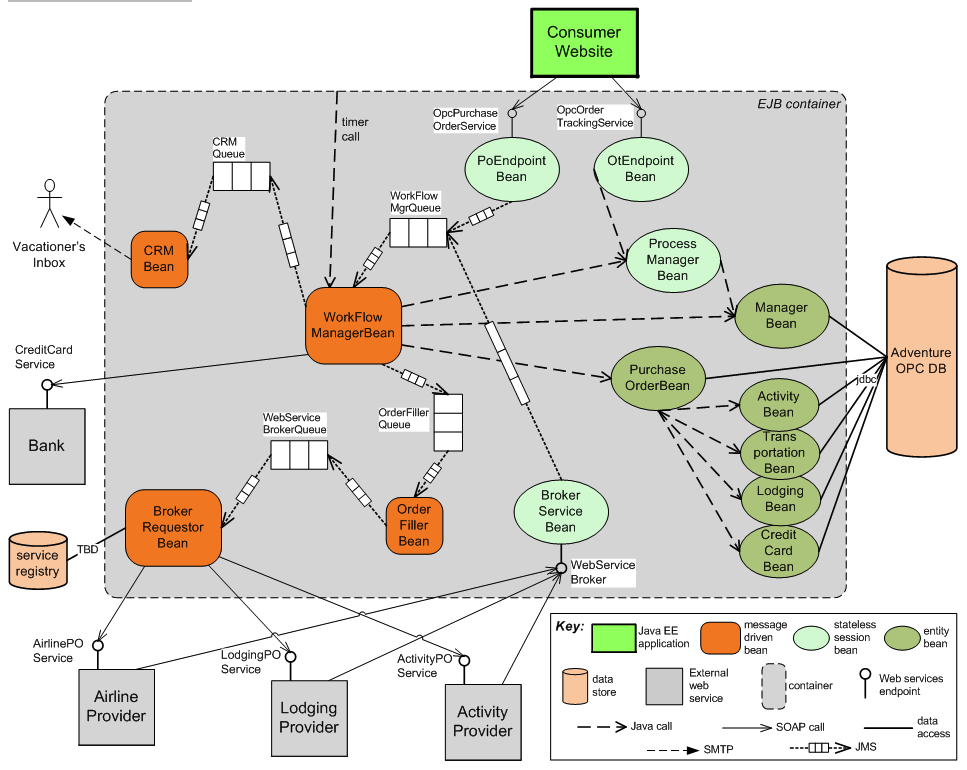
\includegraphics[width=120mm]{../AdventureBuilderCandC}
	\end{center}
	
	The views \textbf{does not} use the architectural style

   	\optionA{Per-to-peer}
	\optionB{Shared-data}
    \optionC{Communicating processes}
    \optionD{Publish-subscribe}
		
    \putOptions
\end{ClosedQuestion}
}

\newcommand{\qAdventureBuilderFour}{
\begin{ClosedQuestion}
  	Consider the following architectural view of the Adventure Builder system, designed around the Order Processing Center
	
	\begin{center}
		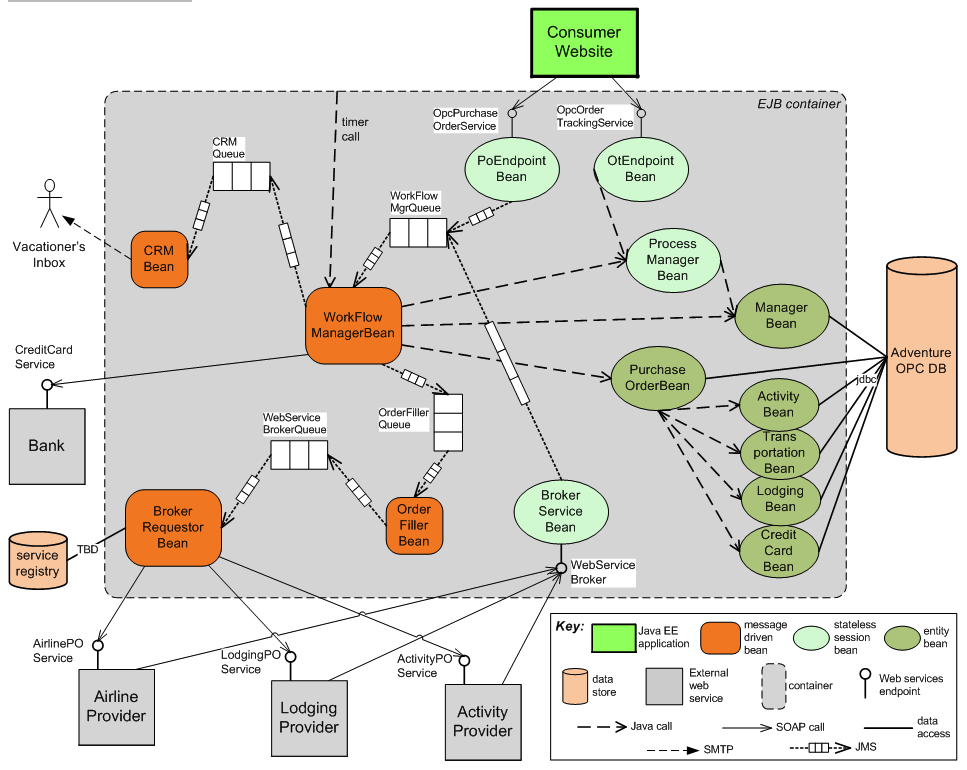
\includegraphics[width=120mm]{../AdventureBuilderCandC}
	\end{center}
	
	The views \textbf{does not} allow the reason about the quality of

   	\optionA{Interoperability}
	\optionB{Modifiability}
    \optionC{Performance}
    \optionD{Security}
		
    \putOptions
\end{ClosedQuestion}
}

% Adventure Builder Two

\newcommand{\qAdventureBuilderFive}{
\begin{ClosedQuestion}
  	Consider the following requirement for availability of the Adventure Builder system
	
	\begin{quote}
		The Consumer Web site sent a purchase order request to the order processing center (OPC). The OPC processed that request but didn't reply to Consumer Web site within five seconds, so the Consumer Web site resends the request to the OPC.
	\end{quote}
	
	If we represent this requirement as a scenario

   	\optionA{The stimulus is an omission and the tactic is retry}
	\optionB{The stimulus is a crash and the tactic is retry}
    \optionC{The stimulus is an incorrect timing and the tactic is ignore faulty behaviour}
    \optionD{The stimulus is incorrect response and the tactic is voting}
		
    \putOptions
\end{ClosedQuestion}
}

\newcommand{\qAdventureBuilderSix}{
\begin{ClosedQuestion}
  	Consider the following requirement for availability of the Adventure Builder system
	
	\begin{quote}
		The Consumer Web site is available to the user 24x7. If an instance of OPC application fails, the fault is detected and the system administrator is notified in 30 seconds; the system continues taking order requests; another OPC instance is automatically created; and data remains in consistent state.
	\end{quote}
	
	In order to support this quality it is necessary to 

   	\optionA{Use a passive redundancy tactic in the OPC (Order Processing Center)}
	\optionB{Use a passive redundancy tactic in the Consumer Web site}
    \optionC{Use an active redundancy tactic in the OPC (Order Processing Center) }
    \optionD{Use an active redundancy tactic in the Consumer Web site}
		
    \putOptions
\end{ClosedQuestion}
}


% Catalog of DVDs

\newcommand{\qDVDCatalogMeta}{
\begin{ClosedQuestion}
	Consider the module viewtype views of the DVD Catalog application. The architect knows about a new requirement 
	
	\begin{quote}
		The application should support other kinds of catalogs (CDs, games, books, ...). 
	\end{quote}
	
	This requirement requires a change of
	
    \optionA{The layered view to support a new specific layer for the customization of the catalog}
    \optionB{The layered view to accommodate a new layer for each kind of catalog, which other layers may use}
    \optionC{The data model view in order to define entities for each kind of catalog}
    \optionD{The data model view in order to define generic entities that can be customized for different kinds of catalogs}
 \putOptions
\end{ClosedQuestion}
}

\newcommand{\qDVDCatalogMobile}{
\begin{ClosedQuestion}
	Consider the module viewtype views of the DVDCatalog application. The architect knows about a new requirement 
	
	\begin{quote}
		To support iPhone/iPad/Android version with sync, which allows offline use of the application in the mobile device and data synchronization to occur when a connection is available
	\end{quote}
	
	This requirement requires a change of
	
    \optionA{The decomposition view to include a module for the synchronization responsibilities}
    \optionB{The uses view to represent how the mobile device uses the Catalog application}
    \optionC{The layered view to include a layer for each type of device}
    \optionD{The domain layer of the layered style to represent the types of devices}
 \putOptions
\end{ClosedQuestion}
}


% Component-and-connector viewtypes

\newcommand{\qAvailabilityINGLES}{
  \begin{ClosedQuestion}
    Suppose that, to satisfy an availability requirement related with
    the occurrence of faults at the network infrastructure used by
    your system, you want to use the tactic named \emph{Ping/Echo}.
    How does the use of that tactic manifests in the architectural
    views of your system?

    \optionA{Only in the Deployment view}
    \optionB{Only in the Decomposition view}
    \optionC{Only in a component-and-connector view}
    \optionD{Both in a component-and-connector and the Deployment
      views}

    \putOptions

% Resposta: D
 \end{ClosedQuestion}
}

\newcommand{\qTiposVistaDesempenhoINGLES}{
  \begin{ClosedQuestion}
    To analyse the performance of a system

    \optionA{Only views of the component-and-connector viewtype are needed}
    \optionB{All viewtypes may be necessary}
    \optionC{Only views of the component-and-connector viewtype and allocation viewtype are needed}
    \optionD{Views of the module viewtype are not needed}
    \putOptions
% Resposta: B
 \end{ClosedQuestion}
}


% Component-and-connector style one

\newcommand{\qPeerToPeerDynamicReconfiguration}{
\begin{ClosedQuestion}
	In the description of the Gnutella system can be read:
	
	\begin{quote}
		The topology of the system changes at runtime as peer components connect and disconnect to the network.
	\end{quote}
	
    \optionA{When a peer connects to the network it establishes connections with all other peers in the network}
    \optionB{The behavior described in the sentence can be represented in a view where the dynamic reconfiguration architectural style is used}
    \optionC{When a peer receives a connection it sends all its files to the peer connecting it}
    \optionD{The behavior described in the sentence can be represented in a view where the tier architectural style is used}
 \putOptions
\end{ClosedQuestion}
}

\newcommand{\qPeerToPeerSpace}{
\begin{ClosedQuestion}
	The Peer-to-Peer architectural style provides high scalability and availability. In the context of a file sharing system  
	
    \optionA{The file transfers follows the same path of nodes used to identify where the file was located}
    \optionB{The peer initiating the request for a file needs to know where the file is located}
    \optionC{If a peer providing a file crashes it is necessary to restart downloading the file from the begin}
    \optionD{The price for high scalability and availability is the need to have several replicas of the files to be shared}
 \putOptions
\end{ClosedQuestion}
}



% Component-and-connector style two

\newcommand{\qPipeFilterComposition}{
\begin{ClosedQuestion}
	The Pipe-and-Filter style allows composition of filters 
	
    \optionA{But when the filters are executed sequentially the composition power is reduced}
    \optionB{Which improves modifiability, because filters are decoupled through pipes}
    \optionC{But the size of buffers may reduce the composition power}
    \optionD{And filters do not have to agree on the data formats}
 \putOptions
\end{ClosedQuestion}
}

\newcommand{\qTresTiersINGLES}{
  \begin{ClosedQuestion}
    Currently, the most popular architecture for an enterprise
    application is composed of 3 tiers.  The three tiers are

    \optionA{The presentation logic layer, domain logic layer, and
      data access layer}
    \optionB{The traditional web applications, the mashups, and the rich internet applications (RIAs)}
    \optionC{The web browser, o web server, and the data base}
    \optionD{The web services layer, the domain logic layer, and the
      data access layer}
    \putOptions

% Resposta: C
  \end{ClosedQuestion}
}


% Component-and-connector style three

\newcommand{\qSOAINGLES}{
  \begin{ClosedQuestion}
    In the Service Oriented Architecture style it is common to have a
    specialized component, named \emph{Enterprise Service Bus} (ESB).
    The goal of using of an ESB in a system is

    \optionA{To facilitate the interaction among heterogeneous
      components that use distinct communication protocols}
    \optionB{To promote the use of a common communication protocol for
      all the remaining components of the system}
    \optionC{To increase the performance of the interaction between
      the components of the system}
    \optionD{To create a strong coupling between the various services
      provided by the organization}

    \putOptions

% Resposta: A
 \end{ClosedQuestion}
}

\newcommand{\qSOAInteroperability}{
\begin{ClosedQuestion}
	The Service-Oriented Architecture style improves interoperability because
	
    \optionA{It enforces the use of a single implementation language among all applications}
    \optionB{The orchestration is in charge of improving the transparent location of service providers}
    \optionC{The enterprise service bus coordinates the execution of several services}
    \optionD{It decouples applications developed for different organizations}
 \putOptions
\end{ClosedQuestion}
}

% Component-and-connector style four

\newcommand{\qWhiteBoxTestingINGLES}{
  \begin{ClosedQuestion}
    Consider the following excerpt from the Wikipedia page on
    \emph{white-box testing}:
    \begin{quote}
      White-box testing is a method of testing software that tests
      internal structures or workings of an application, as opposed to
      its functionality. In white-box testing an internal perspective
      of the system (including the module's code), as well as
      programming skills, are required and used to design test
      cases. The tester chooses inputs to exercise paths through the
      code and determine the appropriate outputs.
    \end{quote}
  
    Assuming that you belong to the team testing a complex system and
    that you are responsible for performing white box tests on the
    system, which of the following architectural views of the system
    would be most useful to you?

    \optionA{Work Assignment views}
    \optionB{Generalization views}
    \optionC{Deployment views}
    \optionD{Implementation views}
    \putOptions

  \end{ClosedQuestion}
}

\newcommand{\qInstallView}{
\begin{ClosedQuestion}
  Consider a system that will require a significative configuration effort during deployment, because it provides several variations of the same functionalities and it is necessary to choose which functionalities better fit in each case. The most helpful architectural view for this situation is
 
  \optionA{Work assignment view}
  \optionB{Install view}
  \optionC{Implementation view}
  \optionD{Deployment view}
 \putOptions
\end{ClosedQuestion}
}

% Component-and-connector style five

\newcommand{\qArqChrome}{
\begin{ClosedQuestion}
	The Chromium is a web browser that introduced an innovative architecture. In the Chromium description we can read:
 
  \begin{quote}
    We use separate processes for browser tabs to protect the overall
    application from bugs and glitches in the rendering engine.  We
    also restrict access from each rendering engine process to others
    and to the rest of the system.  In some ways, this brings to web
    browsing the benefits that memory protection and access control
    brought to operating systems.

    We refer to the main process that runs the UI and manages tab and
    plugin processes as the "browser process" or "browser."  Likewise,
    the tab-specific processes are called "render processes" or
    "renderers."  The renderers use the WebKit open-source layout
    engine for interpreting and laying out HTML.
  \end{quote}
  
  Which architectural style should we use to represent this aspect of Chromium?

    \optionA{Communicating Processes}
    \optionB{Client-Server}
    \optionC{Peer-to-Peer}
    \optionD{Uses}
  \putOptions
\end{ClosedQuestion}
}

\newcommand{\qChromeMultiPlatform}{
\begin{ClosedQuestion}
	The Chromium is a web browser that introduced an innovative architecture. In the Chromium description we can read:

  \begin{quote}
    Chromium is a large and complex cross-platform product.  We try to
    share as much code as possible between platforms, while
    implementing the UI and OS integration in the most appropriate way
    for each.  While this gives a better user experience, it adds
    extra complexity to the code.  This document describes the
    recommended practices for keeping such cross-platform code clean.

    We use a variety of different file naming suffixes to indicate
    when a file should be used:
    \begin{itemize}
    \item Windows files use the \texttt{\_win} suffix.
    \item Cocoa (Mac UI) files use the \texttt{\_cocoa} suffix, and lower-level Mac files use the \texttt{\_mac} suffix.
    \item Linux files use \texttt{\_linux} for lower-level files, \texttt{\_gtk} for GTK-specific files, and \texttt{\_x} for X Windows (with no GTK) specific files.
    \item Posix files shared between Mac and Linux use the \texttt{\_posix} suffix.
    \item Files for Chrome's ``Views'' UI (on Windows and experimental GTK) layout system use the \texttt{\_views} suffix.
   \end{itemize}

    The separate front-ends of the browser are contained in their own directories:
    \begin{itemize}
    \item Windows Views (and the experimental GTK-views): \\
      \texttt{chrome/browser/ui/views}
    \item Linux GTK: \texttt{chrome/browser/gtk}
    \item Mac: \texttt{chrome/browser/cocoa}
    \end{itemize}
  \end{quote}
  
  Which architectural style should we use to represent this aspect of Chromium?

    \optionA{Implementation}
    \optionB{Work assignment}
    \optionC{Decomposition}
    \optionD{None, because this description does not describe any architectural aspect of the system}
  \putOptions
\end{ClosedQuestion}
}

% Twitter - Timelines of Scale - Scenario

\newcommand{\qTwitterOne}{
\begin{ClosedQuestion}
	Consider the following description of the behavior of Twitter ingestion mechanisms
	
	\begin{quote}
		Write. when a tweet  comes in there's an O(n) process to write to Redis clusters, where n is the number of people following you. Painful for Lady Gaga and Barack Obama where they are doing 10s of millions of inserts across the cluster. All the Redis clusters are backing disk, the Flock cluster stores the user timeline to disk, but usually timelines are found in RAM in the Redis cluster.
	\end{quote}
	
	\optionA{The quality being addressed is performance and the tactic multiple copies of data}
	\optionB{The quality being addressed is performance and the tactic multiple copies of computation}
	\optionC{The quality being addressed is performance and the tactics multiple copies of data and multiple copies of computation}
	\optionD{The quality being addressed is availability and the tactic passive redundancy}
	
	\putOptions
\end{ClosedQuestion}
}

\newcommand{\qTwitterTwo}{
\begin{ClosedQuestion}
	Consider the following description of the behavior of Twitter
	
	\begin{quote}
		Solution is a write based fanout approach. Do a lot of processing when tweets arrive to figure out where tweets should go. This makes read time access fast and easy. Don't do any computation on reads. With all the work being performed on the write path ingest rates are slower than the read path, on the order of 4000 QPS.
	\end{quote}
	
	To describe this behavior we need to 
	
	\optionA{Write a single scenario on performance}
	\optionB{Write two scenarios on performance}
	\optionC{Write a scenario on performance and a scenario on interoperability}
	\optionD{Write a single scenario on interoperability}
	
	\putOptions
\end{ClosedQuestion}
}


% Twitter - Timelines of Scale - Tactic

\newcommand{\qTwitterThree}{
\begin{ClosedQuestion}
	Consider the following description of the behavior of Twitter
	
	\begin{quote}
		Solution is a write based fanout approach. Do a lot of processing when tweets arrive to figure out where tweets should go. This makes read time access fast and easy. Don't do any computation on reads. With all the work being performed on the write path ingest rates are slower than the read path, on the order of 4000 QPS.
	\end{quote}
	
	To describe the performance quality of this behavior, and considering that the number of reads is much higher than the number of writes, we need to have a view that includes
	
	\optionA{Tiers style}
	\optionB{Client-server style}
	\optionC{Shared-data style}
	\optionD{Pipe-and-filter style}
	
	\putOptions
\end{ClosedQuestion}
}

\newcommand{\qTwitterFour}{
\begin{ClosedQuestion}
	Consider the following description of the behavior of Twitter ingestion mechanisms
	
	\begin{quote}
		Write. when a tweet  comes in there's an O(n) process to write to Redis clusters, where n is the number of people following you. Painful for Lady Gaga and Barack Obama where they are doing 10s of millions of inserts across the cluster. All the Redis clusters are backing disk, the Flock cluster stores the user timeline to disk, but usually timelines are found in RAM in the Redis cluster.
	\end{quote}
	
	The view that represents this behavior should be of the
	
	\optionA{Module viewtype}
	\optionB{Component-and-connector viewtype}
	\optionC{Install architectural style of the allocation viewtype}
	\optionD{It is not necessary to represent this behavior because it does not describe any qualities}
	
	\putOptions
\end{ClosedQuestion}
}

% Microservices

\newcommand{\qMicroservicesOne}{
\begin{ClosedQuestion}
	Consider the Microservice architectural style. Which of the following sentences \textbf{does not} describe an advantage of microservices?
			
    \optionA{Each service can be developed and deployed independently}
    \optionB{Easier to scale development}
    \optionC{Eliminates any long-term commitment to a technology stack}
    \optionD{Testing is easier}
 \putOptions 
\end{ClosedQuestion}
}

\newcommand{\qMicroservicesTwo}{
\begin{ClosedQuestion}
	Consider the following definition of Microservice architectural style by Martin Fowler
	
	\begin{quote}
		The microservice architectural style is an approach to developing a single application as a suite of small services, each running in its own process and communicating with lightweight mechanisms, often an HTTP resource API. These services are built around business capabilities and independently deployable by fully automated deployment machinery. There is a bare minimum of centralized management of these services, which may be written in different programming languages and use different data storage technologies.
	\end{quote}
	
	To represent an architecture based on Microservices 
			
    \optionA{We do not need a view of the module viewtype because it is about the runtime properties of the system}
    \optionB{We do not need a view of the allocation viewtype because deployment is automated}
    \optionC{The component-and-connector view should emphasize the performance qualities of systems following the microservices architecture}
    \optionD{It is necessary to use views of the three viewtypes}
 \putOptions 
\end{ClosedQuestion}
}

% Amazon architecture

\newcommand{\qMicroAndAmazonThree}{
\begin{ClosedQuestion}
	In the interview Werner Vogels from Amazon gives to Jim Gray, Werner Vogels says that
	
	\begin{quote}
		The stored data formats are decoupled from the format in which you communicate data items. If there is no need for sharing schemas of the actual storage layout, you can focus on making sure that the service interfaces can evolve in a way that allows you to handle variations of data formats. 
	\end{quote}
	
	Which means that in the software architecture of Amazon's systems
			
    \optionA{The shared-data architectural style is not applied because data is encapsulated inside services}
    \optionB{The sharing of data is done using a service-oriented architecture}
    \optionC{Modifiability is not a concern of their architecture}
    \optionD{The decouple of data formats does not support scalability because of the transactional properties}
 \putOptions 
\end{ClosedQuestion}
}

\newcommand{\qWorldWideEN}{
  \begin{ClosedQuestion}
	  In world-wide systems like Facebook or Amazon,
	  
      \optionA{All functionalities can be transactional}
      \optionB{Only a small set of functionalities are transactional}
      \optionC{It is not necessary to have transactional properties because all data is in memory}
      \optionD{Only the isolation property of transactions is supported} 
	  

     \putOptions
% Resposta: B
   \end{ClosedQuestion}
}

% Boundaded Contexts and transactional architecture

\newcommand{\qBoundedContextOne}{
  \begin{ClosedQuestion}
	  Consider the following representation of a system following a microservices architecture,
	  
  	\begin{center}
  		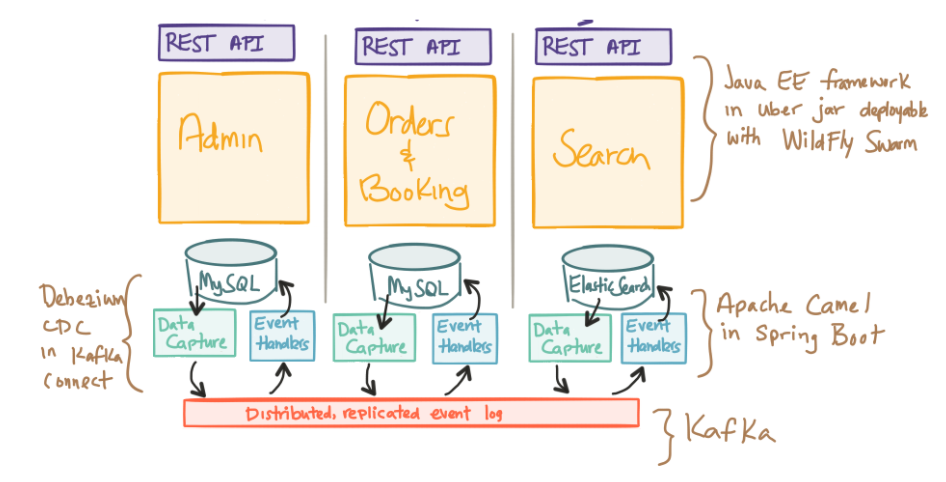
\includegraphics[width=140mm]{../MicroservicesArchitecture}
  	\end{center}
	  
	  After an invocation through the REST API
	  
      \optionA{an ACID transaction occurs in all the involved applications}
      \optionB{a two-phase commit protocol takes place between the involved applications}
      \optionC{a ACID transaction occurs in each of the involved applications, but we can not infer which transaction occurs first}
      \optionD{an ACID transaction occurs in the invoked application and ACID transactions in the other involved applications will eventually occur later} 
	  

     \putOptions
% Resposta: D
   \end{ClosedQuestion}
}

\newcommand{\qBoundedContextTwo}{
  \begin{ClosedQuestion}
	  Consider the following representation of a system following a microservices architecture,
	  
  	\begin{center}
  		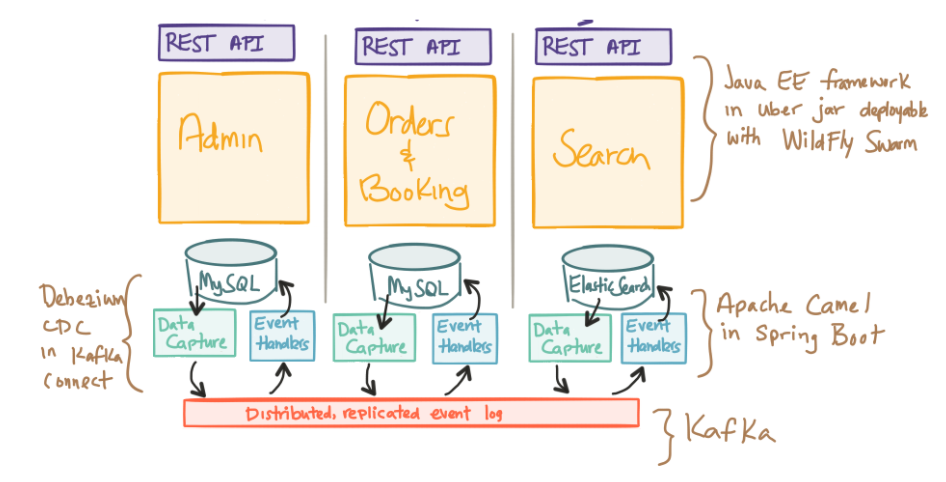
\includegraphics[width=140mm]{../MicroservicesArchitecture}
  	\end{center}
	  
      \optionA{When an event is published to the distributed log, the order of delivery to the different subscribing applications is predefined}
      \optionB{When two events are published to the distributed log they are delivered to the different subscribing applications in the same order}
      \optionC{The distributed log guarantees that events will be delivered only once}
      \optionD{The distributed log may not deliver some of the events that are published to their subscribers} 
	  

     \putOptions
% Resposta: C
   \end{ClosedQuestion}
}

% Effective aggregate design

\newcommand{\qDomainDesignOne}{
  \begin{ClosedQuestion}
	  Consider the following figure
	  
  	\begin{center}
  		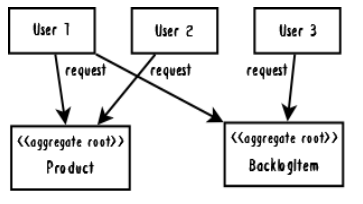
\includegraphics[width=70mm]{../ProductDomainModelTwo}
  	\end{center}
	  
      \optionA{The access to two different aggregate instances in the context of the same request does not hinder scalability}
      \optionB{This is the solution followed by Twitter client applications}
      \optionC{It describes the typical behavior of a microservices system}
      \optionD{To support high scalability the request of \texttt{User 1} needs to be decomposed into a request to only one of the aggregate instances and the processing in the other aggregate occurs in the background} 
	  

     \putOptions
% Resposta: 
   \end{ClosedQuestion}
}

\newcommand{\qDomainDesignTwo}{
  \begin{ClosedQuestion}
	  Consider the following data model
	  
  	\begin{center}
  		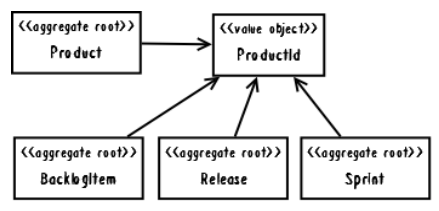
\includegraphics[width=80mm]{../ProductDomainModel}
  	\end{center}
	  
      \optionA{It allows high scalability because the data model has only four entities}
      \optionB{It allows high scalability because it is possible the implement transactions associated to each one of the aggregates}
      \optionC{It allows high scalability because the only synchronized access is to the \texttt{ProductId}, so it requires a single contention point}
      \optionD{It does not allow high scalability} 
	  

     \putOptions
% Resposta: B
   \end{ClosedQuestion}
}






% Fourth Mini-test


% Component-and-connector viewtypes

% Reused with changes
\newcommand{\qComponentConnectorTwo}{
\begin{ClosedQuestion}
	The connectors on component-and-connector view
	
	\optionA{Represent the hardware infrastructure that allows components to communicate
		with each other}
	\optionB{May, on another view of the system, be represented by a set of components
		and connectors}
	\optionC{Represent the dependency relations that exist among the various components}
	\optionD{Represent the control flow during an execution of the system}
	
	\putOptions
\end{ClosedQuestion}
}

% Reused
\newcommand{\qInterfaceDelegation}{
\begin{ClosedQuestion}
	Consider the concept of interface delegation 
		
    \optionA{It corresponds to a particular case of a specialization in a generalization view}
    \optionB{It represents a relation between a connector's role and a port of one of its internal components}
    \optionC{It represents a relation between a component's port and a port of one of its internal components}
    \optionD{It represent a relation between a component's port and a connector's role}
 \putOptions
\end{ClosedQuestion}
}



% Component-and-connector styles

% Reused
\newcommand{\qPipesFilters}{
\begin{ClosedQuestion}
	Consider that you intend to develop a system where it is necessary to change the emails received by the server (for instance, to remove potential virus or URLs for phishing sites). The goal is that each email is processed by this system before it is sent to other servers or it is stored locally. Additionally, the system should be easily modified to support new kinds of transformations. Which style is more suitable to satisfy these requirements? 

    \optionA{Peer-to-Peer}
    \optionB{Pipe-and-Filter}
    \optionC{Client-Server}
    \optionD{Publish-Subscribe}
 \putOptions
\end{ClosedQuestion}
}

% Reused
\newcommand{\qCommunicationProcesses}{
\begin{ClosedQuestion}
	The Java web servers, like Tomcat, use threads to process requests. For each request they create (or reuse) a thread to process it.
	To draw a architectural view that describes this behaviour we should use 
	
    \optionA{A Module viewtype view}
    \optionB{A Allocation viewtype view}
    \optionC{A Communicating processes view}
    \optionD{A Install view}
 \putOptions
\end{ClosedQuestion}
}

% Reused
\newcommand{\qTiers}{
\begin{ClosedQuestion}
	The Tiers architectural style
	
    \optionA{Applies layers to tiers}
    \optionB{Restricts the communication between components because, for instance, a group of components should be located in the same hardware}
    \optionC{Is an extension of the Client-Server architectural style}
    \optionD{Defines tiers as components}
 \putOptions
\end{ClosedQuestion}
}

% Reused - changed
\newcommand{\qPublishSubscribe}{
\begin{ClosedQuestion}
	In the Publish-Subscribe architectural style 
	
    \optionA{A component can subscribe to events}
    \optionB{It is always guaranteed that all the published events are received by their subscribing components}
    \optionC{The events should be delivered by the same order they are sent}
    \optionD{The set of events types are predefined at initialization time}
 \putOptions
\end{ClosedQuestion}
}

% Reused
\newcommand{\qGraphiteViewsOne}{
 \begin{ClosedQuestion}
    In Graphite system  the \emph{receiver} and the \emph{writer threads} support asynchronous writing of metrics to optimize disk accesses. The interaction between these two components follow the architectural style

    \optionA{Client-server}
    \optionB{Communicating Processes}
    \optionC{Repository}
    \optionD{Pipes-and-Filters}

     \putOptions
% Resposta: B
   \end{ClosedQuestion}
}

% Reused
\newcommand{\qGraphiteViewsTwo}{
  \begin{ClosedQuestion}
	  A high-level component-and-connect view of Graphite system can be designed using only the architectural style(s)

    \optionA{Shared-data and Communicating-Processes}
    \optionB{Communicating-Processes}
    \optionC{Tiers}
    \optionD{Client-Server and Shared-data}

     \putOptions
% Resposta: D
   \end{ClosedQuestion}
}


% Adventure Builder

% Reused
\newcommand{\qAdventureBuilderOne}{
\begin{ClosedQuestion}
	Consider the following view of the Adventure Builder system
	
	\begin{center}
		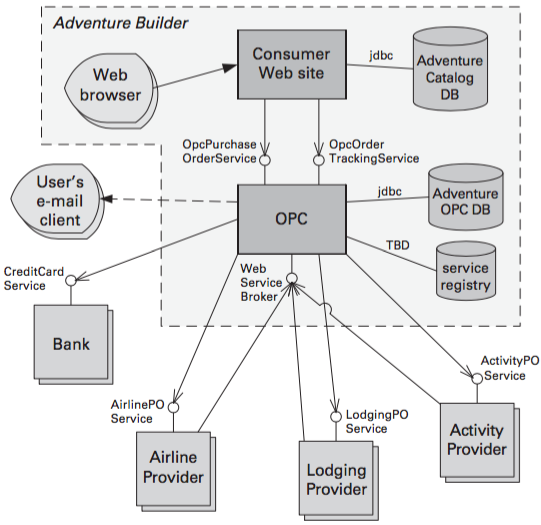
\includegraphics[width=120mm]{AdventureBuilder-SOA}
	\end{center}
	
	In this view the following architectural styles are used
	
		
    \optionA{Service-oriented architecture, and Client-server}
    \optionB{Service-oriented architecture, and Shared-data}
    \optionC{Service-oriented architecture, Shared-data, and Peer-to-peer}
    \optionD{Service-oriented architecture, Shared-data, Peer-to-peer, and Client-server}
 \putOptions 
\end{ClosedQuestion}
}
	
% Reused
\newcommand{\qAdventureBuilderTwo}{
\begin{ClosedQuestion}
	Consider the following view of the Adventure Builder system
	
	\begin{center}
		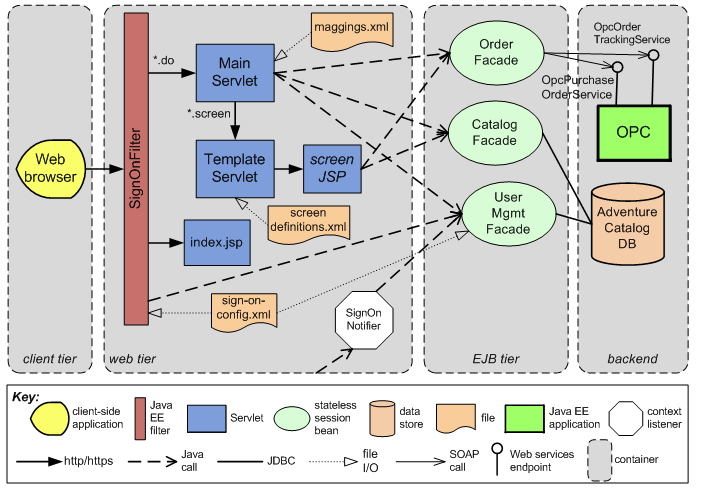
\includegraphics[width=140mm]{AdventureBuilder-Tiers}
	\end{center}
	
	In this view the following architectural styles are used
		
    \optionA{Tiers}
    \optionB{Tiers, and Shared-data}
    \optionC{Tiers, Shared-data, and Service-oriented architecture}
    \optionD{Tiers, Shared-data, Service-oriented architecture, and Client-server}
 \putOptions 
\end{ClosedQuestion}
}




% Third Mini-test


% Architectural Views

% REUSED
\newcommand{\qUsesCalls}{
\begin{ClosedQuestion}
	A function call is not necessarily a uses relation of the Uses architectural style of the Module viewtype because
	
    \optionA{The correctness of the caller module may not depend on the correct implementation of the invoked function in the called module}
    \optionB{The invoked function may not have any input parameter}
    \optionC{The invoked function may not have any output parameter}
    \optionD{The invoked function may not have both any input parameter nor any output parameter}
 \putOptions
\end{ClosedQuestion}
}

\newcommand{\qModuleComponent}{
\begin{ClosedQuestion}
	Consider the kind of relations between components and modules.
		
    \optionA{A module contains the code that executes in a single component and a component executes the code of a single module}
    \optionB{A module contains the code that can execute in several components and a component executes the code of a single module}
    \optionC{A module contains the code that executes in a single component and a component can execute the code of several modules}
    \optionD{A module contains the code that can execute in several components and a component can execute the code of several modules}
 \putOptions
\end{ClosedQuestion}
}


% Module viewtype

% REUSED
\newcommand{\qModuleViewtypeTwo}{
\begin{ClosedQuestion}
	Consider the Uses architectural style of the Module viewtype
		
    \optionA{Cycles in the uses relation between modules are a good sign, because it indicates that several modules should be tested together}
    \optionB{The project manager uses this view to get advice on the incremental development of the system}
    \optionC{The uses relation should be applied to the coarse-grained modules, because it allows to identify circular dependences}
    \optionD{There isn't any relation with the layered architectural style because the allowed-to-use relation is more generic}
 \putOptions 
\end{ClosedQuestion}
}

% REUSED
\newcommand{\qModuleViewtypeThree}{
\begin{ClosedQuestion}
	Consider the Layered architectural style of the Module viewtype
		
    \optionA{The modules inside a layer cannot use other modules in the same layer}
    \optionB{A layer cannot call the layer above}
    \optionC{Each layer defines a virtual machine because it provides a set of cohesive functionalities to the upper layer}
    \optionD{It is possible to have a circular allowed-to-use relationship between several layers}
 \putOptions 
\end{ClosedQuestion}
}

% REUSED
\newcommand{\qAspects}{
\begin{ClosedQuestion}
	An architect is decomposing a system into a set of responsibilities using a view of the Decomposition style. However, she had already to backtrack several times and try new decompositions because she always end up with some responsibility that cannot fit within a single module.
	
    \optionA{This means that in this software system it is not possible to modularize each responsibility in a cohesive module}
    \optionB{She should define finer-grained modules where she splits the unassigned responsibility}
    \optionC{She should try to use a view of the Aspects style, assign this responsibility to a single module and define where it crosscuts the other modules}
    \optionD{She should try to use a view of the Layered style and assign this responsibility to a module in the bottom layer that can be used by all the other modules}
 \putOptions
\end{ClosedQuestion}
}

% REUSED
\newcommand{\qDataModelFacebook}{
\begin{ClosedQuestion}
	In Facebook it is not possible to have the information about more that one bilion users in a single disk. Therefore, a sharding technique is applied, where the persistent information is split between several database servers, and applications are routed to the right servers for queries and updates. To describe this architecture
	
    \optionA{It is not necessary to have any view of the Data Model architectural style because Facebook information has a very simple structure}
    \optionB{It is enough to design a view of the Data Model architectural style at the conceptual level because Facebook information has a very simple structure}
    \optionC{It is enough to design a view of the Data Model architectural style at the logical level because the information will be stored in a relational database}
    \optionD{It is necessary to design a view of the Data Model architectural style at the physical level to deal with performance and consistency issues of the access to data}
 \putOptions
\end{ClosedQuestion}
}


% Adventure Builder

\newcommand{\qAdventureBuilderModuleOne}{
\begin{ClosedQuestion}
	Consider the following modifiability scenario for the Adventure Builder system 
	
	\begin{quote}
		A new business partner (airline, lodging, or activity provider) that uses its own web services interface is added to the system in no more than 10 person-days of effort for the implementation. The business goal is easy integration with new business partners.
	\end{quote}
	
	and the following architectural view
	
	\begin{center}
		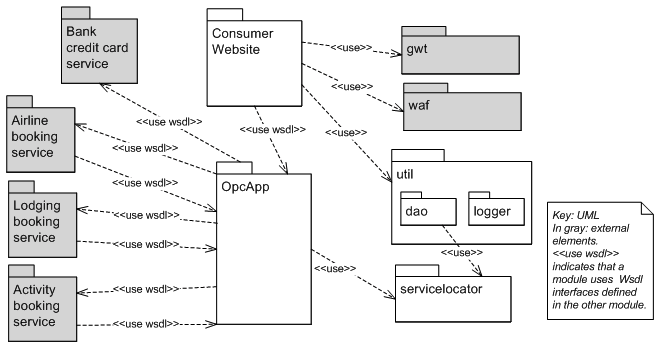
\includegraphics[width=120mm]{AdventureBuilderHighLevelVIew}
	\end{center}
	
    \optionA{The view does not address the scenario}
    \optionB{The view addresses the scenario because it separates the \texttt{Consumer Website} module from the \texttt{OpcApp} module}
    \optionC{The view addresses the scenario because it separates the modules that represent the interfaces a new business partner has to implement}
    \optionD{The view addresses the scenario because the \texttt{Consumer Website} module does not use the interfaces a new business partner has to implement}
 \putOptions
\end{ClosedQuestion}
}

\newcommand{\qAdventureBuilderModuleTwo}{
\begin{ClosedQuestion}
	Consider the following performance/scalability scenario for the Adventure Builder system 
	
	\begin{quote}
		Up to 500 users click to see the catalog of adventure packages following a random distribution over 1 minute; the system is under normal operating conditions; the maximal latency to serve the first page of content is under 5 seconds; average latency for same is less than 2 seconds. If required, the system should easily support an increase in the number of simultaneous requests while maintaining the same latency per request.
	\end{quote}
	
	and the following architectural view
	
	\begin{center}
		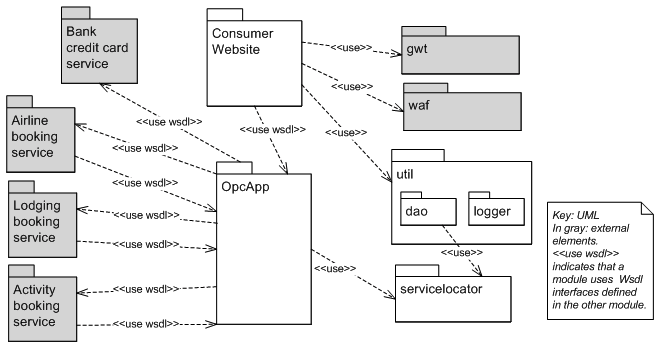
\includegraphics[width=105mm]{AdventureBuilderHighLevelVIew}
	\end{center}
	
    \optionA{The view does not address the scenario}
    \optionB{The view addresses the scenario because it separates the \texttt{Consumer Website} module from the \texttt{OpcApp} module to allow the execution of the \texttt{Consumer Website} module in a component that can have multiple copies of computation}
    \optionC{The view addresses the scenario because it separates the modules that represent the interfaces a new business partner has to implement}
    \optionD{The view addresses the scenario because the \texttt{Consumer Website} module uses the \texttt{gwt} and \texttt{waf} modules}
 \putOptions
\end{ClosedQuestion}
}

% Catalog of DVDs

\newcommand{\qDVDCatalogMultiPlatform}{
\begin{ClosedQuestion}
	Consider the module viewtype views of the DVDCatalog application. The architect knows about a new requirement 
	
	\begin{quote}
		To support multi-platform (Mac, Windows, Linux)
	\end{quote}
	
	This requirement requires a change of
	
    \optionA{The layered view to deal with the aspects of portability}
    \optionB{The uses view to show the coupling between the different platforms}
    \optionC{The uses view to show the uses relationships between the different platforms}
    \optionD{The data model view to represent each one of the platforms}
 \putOptions
\end{ClosedQuestion}
}

\newcommand{\qDVDCatalogAspects}{
\begin{ClosedQuestion}
	Consider the module viewtype views of the DVDCatalog application. The architect knows about a new requirement 
	
	\begin{quote}
		To allow the share of catalogs with family and friends, including some access control. 
	\end{quote}
	
	This requirement requires 
	
    \optionA{A change to the uses view to represent that friends can use each other catalog}
    \optionB{A change of the layered view to support different presentations, one for each friend}
    \optionC{A change of the decomposition view to include a set of new modules with the responsibilities associated with the access control}
    \optionD{A new aspect view that includes a module with the responsibilities associated with the access control and that crosscuts some of the other modules}
 \putOptions
\end{ClosedQuestion}
}



% Second Mini-test


% Availability

% REUSED BUT CHANGED
\newcommand{\qOmissionRetry}{
\begin{ClosedQuestion}
	Considering the availability architectural quality, the tactic of retry

    \optionA{Can be applied to any kind stimulus in availability scenarios}
    \optionB{Is useful to support scenarios where the stimulus is an omission}
    \optionC{Can guarantee that the system will not become unavailable}
    \optionD{When applied it increases the latency of the availability scenario's response time}
 \putOptions 
\end{ClosedQuestion}
}

% REUSED
\newcommand{\qAvailability}{
  \begin{ClosedQuestion}
    There are several tactics to satisfy availability requirements,
    which may be applied depending on the concrete requirement that we
    want to satisfy.  Assuming that you want to detect faults of type
    \emph{response} in your system, which tactic is more adequate?

    \optionA{The Ping/Echo tactic}
    \optionB{The Heartbeat tactic}
    \optionC{The Voting tactic}
    \optionD{The Removal from Service tactic}

    \putOptions

% Resposta: C
 \end{ClosedQuestion}
}

% Performance

% REUSED BUT CHANGED
\newcommand{\qScalability}{
  \begin{ClosedQuestion}
    Several of the cases studied in this course have scalability
    requirements.  That means that those systems should be designed in
    such a way that they

    \optionA{Have high throughput}
    \optionB{Have low latency}
    \optionC{Allow many simultaneous users}
    \optionD{May be easily changed to increase their storage capacity}

    \putOptions

% Resposta: D
 \end{ClosedQuestion}
}

% REUSED BUT CHANGED
\newcommand{\qPerformance}{
\begin{ClosedQuestion}
	Consider a scenario for performance where the arrival of events is stochastic with a distribution where there are peeks of events but the arrival of events over a long period is uniform. The best tactic to apply is
		
    \optionA{Manage sampling rate}
    \optionB{Limit event response}
    \optionC{Prioritize events}
    \optionD{Bound execution time}
 \putOptions 
\end{ClosedQuestion}
}



% Modifiablity

\newcommand{\qModifiabilityOne}{
\begin{ClosedQuestion}
	In a modifiability scenario the environment can be characterized as design time, compile time, build time, initiation time, and runtime.
	
    \optionA{When the environment is design time it means that the change should be done before the system enters into production}
    \optionB{When the environment is build time it means that it is necessary to codify a new module that is added by rebuilding the system}
    \optionC{When the environment is initiation time it means that it is necessary to restart the system for the change to effect}
    \optionD{When the environment is runtime the cost of doing the change is higher than in the other environments}
 \putOptions 
\end{ClosedQuestion}
}

\newcommand{\qModifiabilityTwo}{
\begin{ClosedQuestion}
	Consider that a module, that contains a complex business logic, needs to invoke a remote entity using a particular communication protocol and it is needs to manage the invocation, like deal with the possible errors, delays and omissions in the invocation, transform the data before sending it, etc. Which tactic should be applied for a scenario where there will be changes in the communication protocol. Note that the business logic comprises a set of functionalities that is independent of the remote invocation technological aspects. 
			
    \optionA{Encapsulate the module such that the clients of the module should not be aware of the remote invocations}
    \optionB{Use an intermediary that contains all the code associated with the remote invocation separating it from the modules' business logic}
    \optionC{Refactor the common parts between the business logic and the remote invocation}
    \optionD{Increase the semantic coherence between the business logic code and the remote invocation code}
 \putOptions 
\end{ClosedQuestion}
}



% Graphite

% REUSED
\newcommand{\qGraphiteScenarioTacticsOne}{
  \begin{ClosedQuestion}
    In the Graphite system the component \emph{carbon} provides to \emph{webapp} components an access interface to the \emph{buffers} in order to improve the quality of

    \optionA{Performance}
    \optionB{Interoperability}
    \optionC{Availability (Reliability)}
    \optionD{Security}

     \putOptions
% Resposta: C
   \end{ClosedQuestion}
}

% REUSED
\newcommand{\qGraphiteScenarioTacticsTwo}{
  \begin{ClosedQuestion}
	  Which quality, or qualities, of the Graphite system are described by the sentence: \emph{Graphite's Composer UI provides a point-and-click method to create a graph from which you can simply copy and paste the URL}

    \optionA{Usability and Performance}
    \optionB{Usability}
    \optionC{Performance}
    \optionD{Testability}

     \putOptions
% Resposta: B
   \end{ClosedQuestion}
}



% Hadhoop

% REUSED
\newcommand{\qHadoopCheckpoint}{
  \begin{ClosedQuestion}
    In the HDFS system when the \emph{CheckpointNode} and the \emph{NameNode} are deployed in different nodes, the \emph{CheckpointNode} provides:
    \optionA{Performance and availability qualities}
    \optionB{Performance qualities only}
    \optionC{Availability qualities only}
    \optionD{Performance and security qualities}

    \putOptions
% Resposta: A
 \end{ClosedQuestion}
}

% REUSED BUT CHANGED
\newcommand{\qHadoopNameNodeReplica}{
  \begin{ClosedQuestion}
    The architecture of the HDFS system only allows the existence of
    one NameNode.  Given the responsibilities of this component and
    the current architecture of HDFS, what would be the consequences
    of adding the possibility of having replicas of the NameNode in
    the system?

    \optionA{The system would respond faster to all the
      clients' requests}
    \optionB{The performance of the system would not change}
    \optionC{The system would respond faster to requests about
      file locations}
    \optionD{The system would respond faster to requests made by
      DataNodes to update the metadata}
    \putOptions
% Resposta: B
  \end{ClosedQuestion}
}





% First Mini-test

% Software Architecture

% REUSED
\newcommand{\qSoftwareArchitecture}{
\begin{ClosedQuestion}
  The software architecture of a system

    \optionA{Depends mostly on the system's functional requirements}
    \optionB{Depends more on the architect's experience than on anything else}
    \optionC{Should not depend on the skills of the developing team}
    \optionD{None of the above}
 \putOptions
\end{ClosedQuestion}
}

% REUSED
\newcommand{\qEarlyDecisions}{
\begin{ClosedQuestion}
	In his article, \emph{Who Needs and Architect?}, Martin Fowler cites Ralph Johnson definition:
	
	\begin{quote}
		Architecture is the set of decisions that must be made early in a project.
	\end{quote}
	
	In his opinion:
		
    \optionA{This is right because if you don't the project fails}
    \optionB{This is wrong because you can easily change these decisions during the project lifetime}
    \optionC{This is right but you cannot be completely sure whether the decisions are the right ones}
    \optionD{This is wrong because it is against the agile way of thinking the software development process}
 \putOptions
\end{ClosedQuestion}
}


% Requirements

% REUSED
\newcommand{\qGeneralScenario}{
\begin{ClosedQuestion}
	A general scenario for a quality attribute

    \optionA{Describes a concrete quality that a particular system has to implement}
    \optionB{Enumerates, for each kind of quality attribute, all the possible types of source of stimulus, stimulus, response, etc}
    \optionC{Can omit some of the elements like, for instance, the environment, if they are not relevant for the general scenario}
    \optionD{Is a very reusable scenario that can be effectively used in many different concrete situations}
 \putOptions 
\end{ClosedQuestion}
}

% NEW
\newcommand{\qArchitecturalTactics}{
\begin{ClosedQuestion}
	An architectural tactic for a system describes

    \optionA{A non-functional requirement a system has to achieve}
    \optionB{How to control the response to one or more stimulus}
    \optionC{What should be the system response in the occurrence of a stimulus}
    \optionD{A decomposition of the system that fulfills an architectural quality}
 \putOptions 
\end{ClosedQuestion}
}


% Timelines of Scale

\newcommand{\qTwitterScaleOne}{
\begin{ClosedQuestion}
	In the description of the Twitter system we can read:
	
	\begin{quote}
		 Twitter is optimized to be highly available on the read path on the home timeline. Read path is in the 10s of milliseconds.
	\end{quote}
	
	This is achieved because:

    \optionA{The writing of a tweet is a synchronous process where different users have a consistent view of the sequence of tweets}
    \optionB{A tweet is written in each one of the Twitter's servers}
    \optionC{The tweet unique ID is written in the home timeline of each one of the writer's followers}
    \optionD{The tweet content is written in the home timeline of each one of the writer's followers}
 \putOptions 
\end{ClosedQuestion}
}

\newcommand{\qTwitterScaleTwo}{
\begin{ClosedQuestion}
	In the description of the Twitter system we can read:
	
	\begin{quote}
		On the search timeline:
		 Write. when a tweet comes in and hits the Ingester only one Early Bird machine is hit. Write time path is O(1). A single tweet is ingested in under 5 seconds between the queuing and processing to find the one Early Bird to write it to.
	\end{quote}
	
    \optionA{The search timeline is the most important business use case for Twitter}
    \optionB{The ingestion process includes tokenizing of the tweet to include in an index}
    \optionC{The Early Bird server contains the tweet content}
    \optionD{The write in the Early Bird server is synchronous, only when it finishes does the user receives the feedback of a successful post}
 \putOptions 
\end{ClosedQuestion}
}



% Architectures for scalable web applications

\newcommand{\qProxyServer}{
\begin{ClosedQuestion}
	Consider the following figure that presents a Proxy Server, which collapses requests from different users.
	
	\begin{center}
		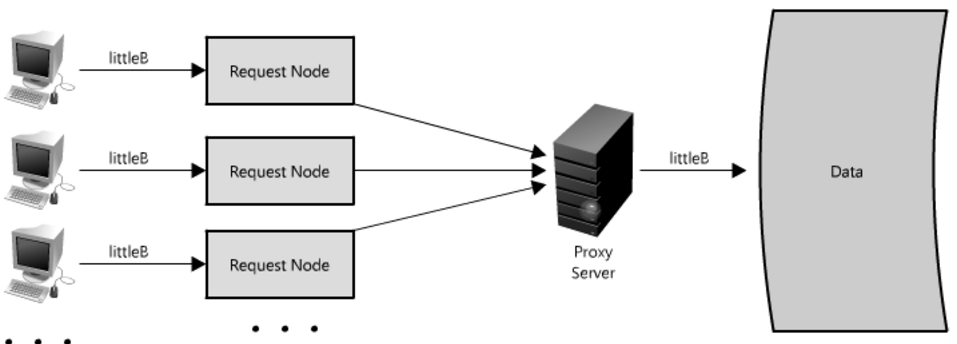
\includegraphics[width=120mm]{ProxyServer}
	\end{center}
	
	
    \optionA{This solution optimizes the performance in terms of the latency of each request}
    \optionB{This solution allows an "infinite"\ increase of the number clients by allowing the inclusion of more Request Nodes}
    \optionC{This solution continues to provide service even if a crash occurs in the Data server}
    \optionD{This solution optimizes the performance in terms of the throughput of processed requests}
 \putOptions 
\end{ClosedQuestion}
}


\newcommand{\qQueues}{
\begin{ClosedQuestion}
	Consider the following figure that presents a Queue where client applications write their requests to be served by a server.
	
	\begin{center}
		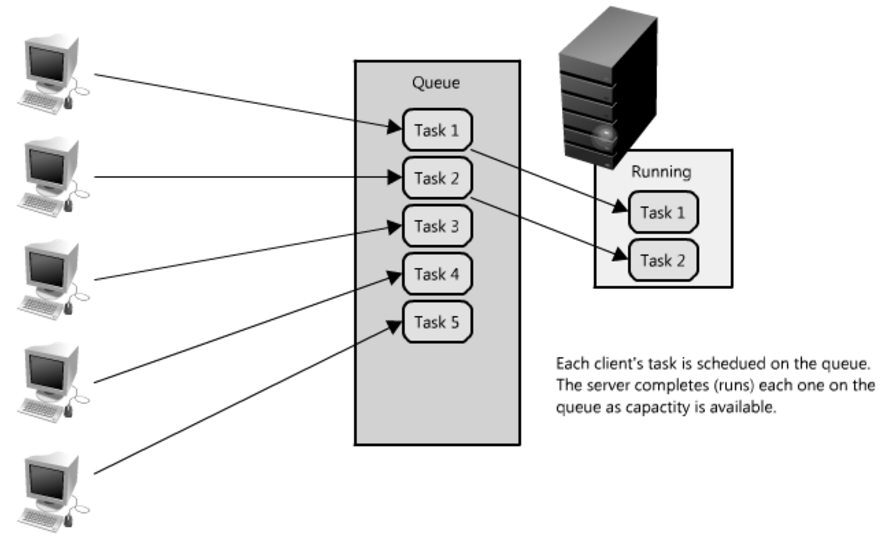
\includegraphics[width=130mm]{Queues}
	\end{center}
	
	
    \optionA{This solution assures a consistency view to the clients of the data that is written}
    \optionB{In this solution the clients invocations have to be synchronous}
    \optionC{In this solution the tasks in the queue need to be sequentially processed, only when a task is finished can another start to be processed}
    \optionD{This solution allows the dimensioning of the number of activities (threads or processes) that run in the server, taking into consideration the server's hardware capacity, in order to have a efficient usage of the server's CPU}
 \putOptions 
\end{ClosedQuestion}
}




% Hadoop


\newcommand{\qHadoopCluster}{
\begin{ClosedQuestion}
	Consider the following figure that presents the Hadoop cluster topology.
	
	\begin{center}
		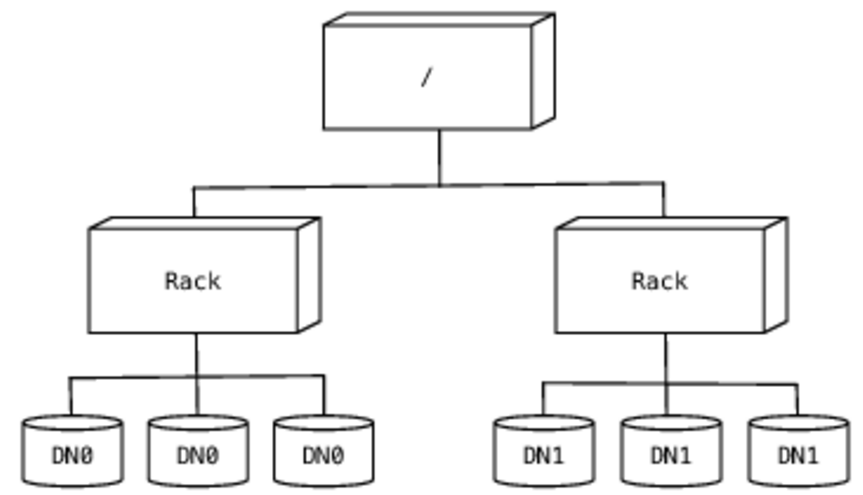
\includegraphics[width=100mm]{HadoopClusterTopology}
	\end{center}
	
    \optionA{When a new block is created, the first replica is written in the node where the writer is located, to improve availability}
    \optionB{When a new block is created, the second replica is not stored in the same rack than the first replica to increase the availability when a Data Node fails}
    \optionC{When a new block is created, the third replica is stored in the same rack than the second replica to improve the performance of reads}
    \optionD{When a read occurs, the client, if it is located in the cluster, receives a list of the DataNodes where the replicas are, ordered by its closeness to the client, to improve performance of reads}
 \putOptions 
\end{ClosedQuestion}
}

\newcommand{\qHadoopCreateFile}{
\begin{ClosedQuestion}
	In the description of Hadoop we can red.
	
	\begin{quote}
		The CheckpointNode periodically combines the existing checkpoint and journal to create a new checkpoint and an empty journal. The CheckpointNode usually runs on a different host from the NameNode since it has the same memory requirements as the NameNode.
	\end{quote}
	
    \optionA{The periodic rebuild of the checkpoint is done to increase the availability of the NameNode}
    \optionB{The advantage of running the CheckpointNode in a different host is to not degrade the availability of the NameNode during checkpoint construction}
    \optionC{The periodic rebuild of the checkpoint improves the performance of the NameNode during normal operation}
    \optionD{The periodic rebuild of the checkpoint improves the performance of the NameNode during its initialization}
 \putOptions 
\end{ClosedQuestion}
}




